\documentclass{article}
\usepackage{hyperref}
\usepackage {graphicx, amsmath}
\usepackage[margin=1.0in]{geometry}
\title{F24 CSE220 Lab1}
\author{
  Andrew Bruce \\ \href{mailto:acbruce@ucsc.edu}{acbruce@ucsc.edu} \and
  Mohit Agrawal \\ \href{mailto:mmagrawa@ucsc.edu}{mmagrawa@ucsc.edu}
}

\begin{document}
\maketitle

\section*{Results}
\subsection*{IPC}
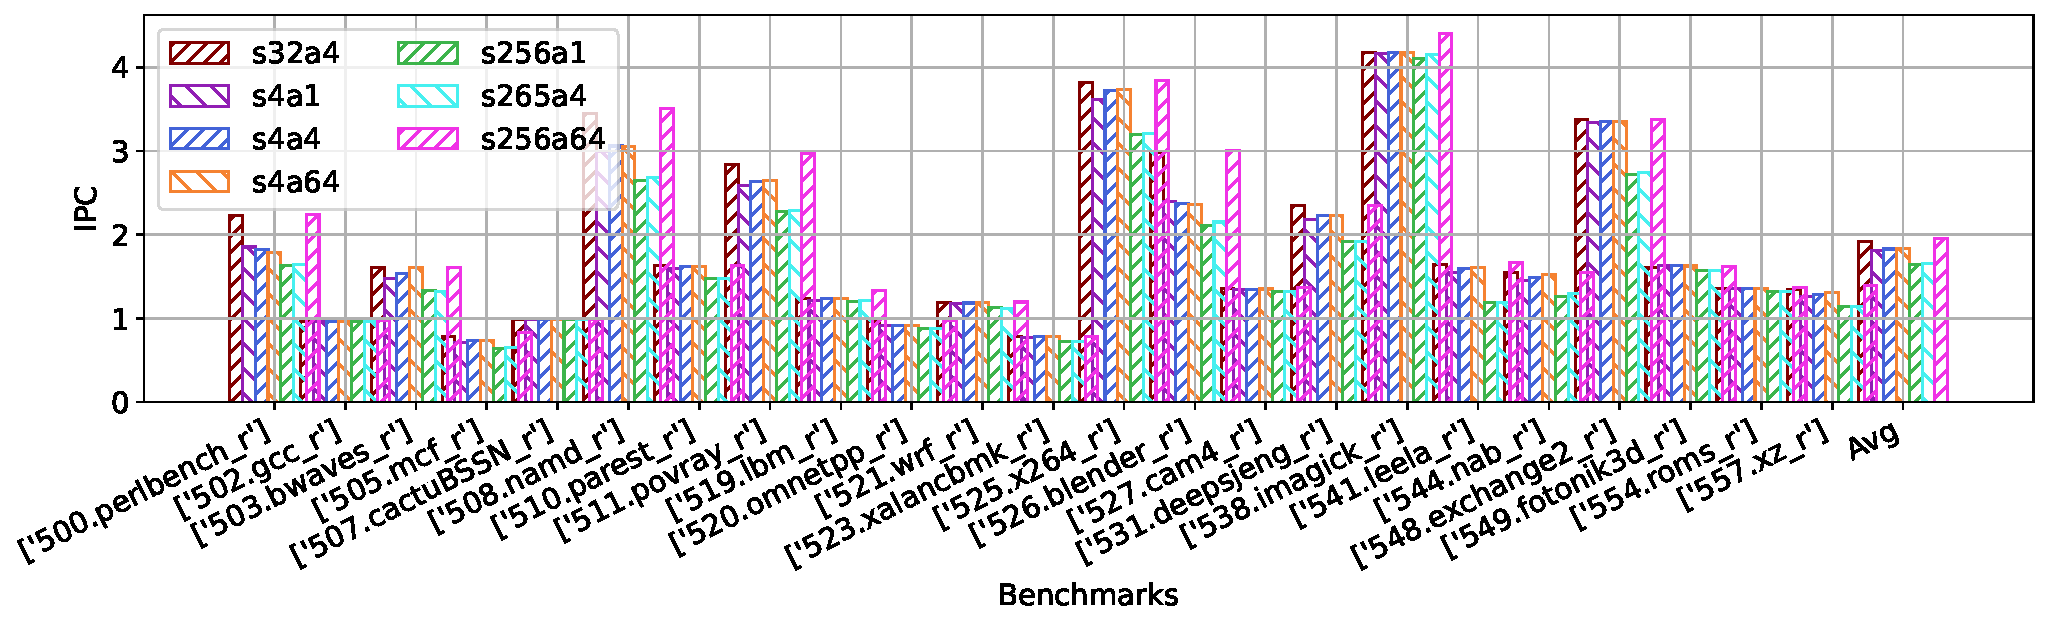
\includegraphics[width=\textwidth]{IPC.pdf}.
We can see that that two pairs of configurations result in roughly the same performance. First we notice that the two configurations with width at 2 have approximately the same IPC of 1 while the 2 configurations with width at 10 have approximately the same IPC of 2. One possible reason the superscalar width increasing by 5 does not result in5 times the IPC, is due to data dependencies not allowing 100\% efficient theoretical pipe-lining according to Amdahl's Law. Increasing the number of cycles for the mapping unit in the pipeline slows down the average IPC by a little bit. One possibility is the slowdown is caused by the increase in pipeline length due to the extra stages dedicated to register renaming.
\subsection*{Branch Misprediction}
\includegraphics[width=\textwidth]{BP.pdf}.
Here we see that all of the configurations have the same branch misprediction percentage. This is because branch miss prediction and its hazard control is determined by how the branch prediction is handled in the architecture, and in this implementation is not something that is changed by the cycle latency or the width as the miss ratio percentage changes based on the technique used to do branch predictions.
\subsection*{DCache miss rate}
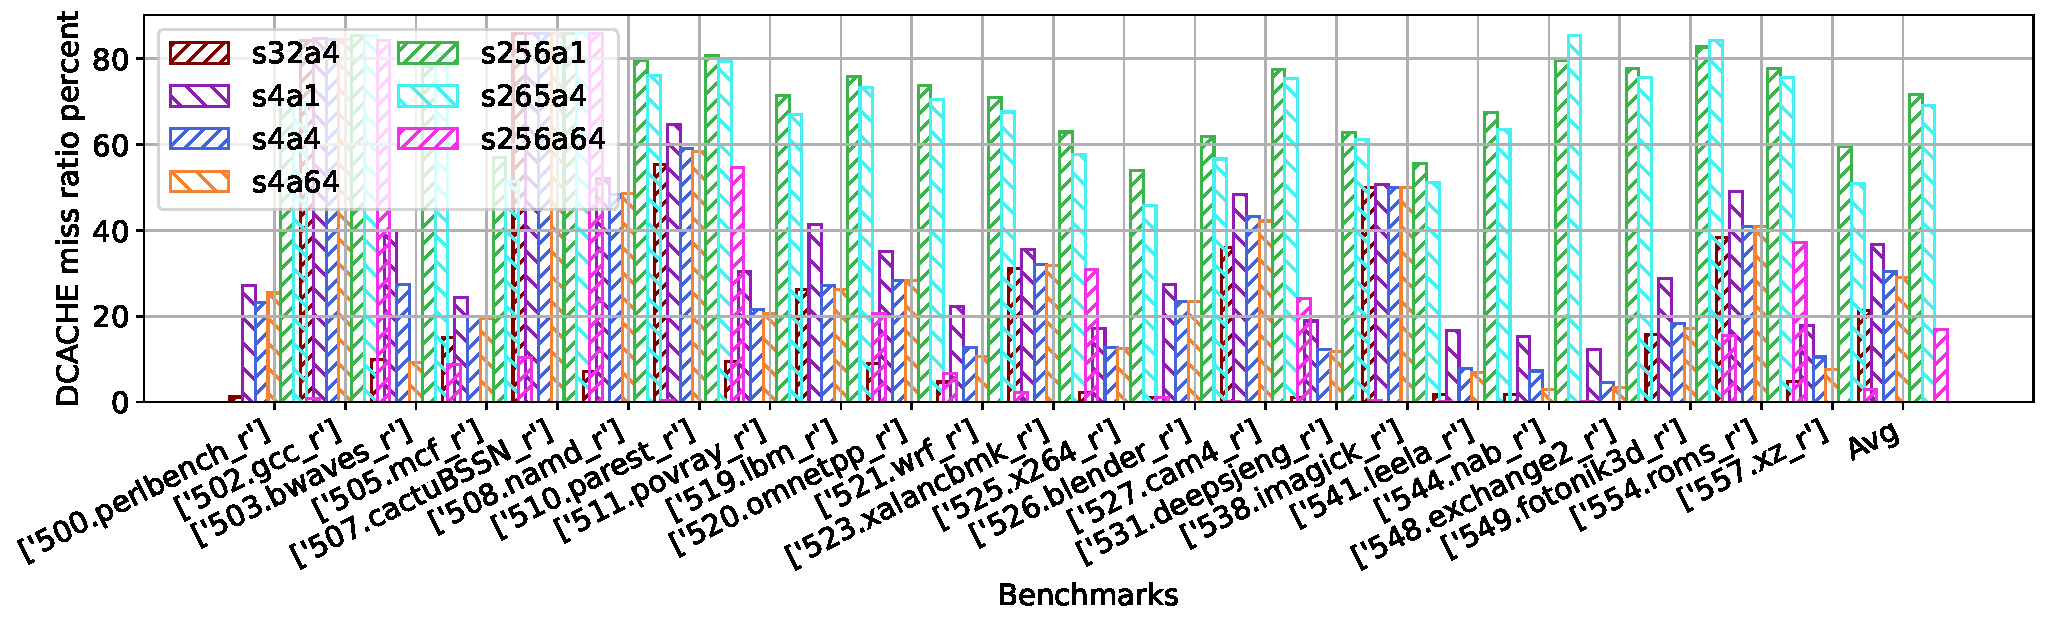
\includegraphics[width=\textwidth]{DCACHE.pdf}.
We again have two pairs of configuration that result in approximately the same average. The two configurations with width of size 10 have a Data Cache (Dcache) miss percentage of 20 while the two configurations with width of size 2 have a miss percentage of 10. Cache miss ratio is determined by the number of Dcache misses over the number of Dcache requests. The Dcache requests will be the same regardless of the configuration as that is determined by the programs instructions and not the architecture. A possible reason the 10 width configuration results in double the number of misses is cache contention which is where you have two instructions trying to fetch the same data at the same time. The Sunny Cove architecture does seem to have a method for dealing with this contention with something called multi-ported caches, however when you increase the width to 10 it can go beyond what the cache is capable of handling at once and therefore it ends ups forcing an instruction to go to slower memory levels resulting in a cache miss. At lower widths the architecture would be able to handle this issue much better which is why it has half the Data cache miss rate. 
\subsection*{ICache miss rate}
\includegraphics[width=\textwidth]{ICACHE.pdf}.
A similar trend to data cache is noticed here however overall the miss rate is almost none for width 2 while miss rate for width 10 is only 1\%. One possible reason for this is that its simply much less likely for a cache miss to occur in the Instruction cache as instruction fetches are much more predictable as they mostly happen sequentially. Sunny cove also implements pre-fetching which leads to better prediction of instructions however the same issue that we noticed with Dcache can happen here with contention. Overall though Icache misses only seems to be an issue in specific programs and even then they are below 10\%.
\begin{minipage}{\textwidth}
\subsection*{Example Scenario}
Assuming the 2-wide superscalar machine configurations run at 3 times higher clock frequency than the 10-wide ones. Which machine configuration is the fastest?\\
Lets first define our variables:\\
C: Clock speed \\
X: 2-wide superscalar with 3 times clock speed (3C) \\
Y: 10-wide superscalar with base clock speed (C) \\
Performance = IPC x Clock Speed \\
From our IPC graph, the average performance of the 10 width processors was only about twice as much as the 2 width processors despite having 5 times the superscalar width. \\
\begin{center}
  $\text{Throughput}_2 = 1\dfrac{\text{Instructions}}{\text{Cycle}} \times 3C\dfrac{\text{Cycles}}{s} = 3C\dfrac{\text{Instructions}}{s}$ \\
  $\text{Throughput}_{10} = 2\dfrac{\text{Instructions}}{\text{Cycle}} \times C\dfrac{\text{Cycles}}{s} = 2C\dfrac{\text{Instructions}}{s}$
\end{center}
Then we can calculate the speedup:
\begin{center}
  $\text{Speedup} = \frac{\text{Throughput}_2}{\text{Throughput}_{10}} = \dfrac{3C}{2C} = 1.5$
\end{center}
This means we have a 50\% speedup with the 2 width processors with 3 times the clock speed over the 10 width ones with base clock speed. So in this case the 2 width processors (X) would be faster. The depth of the map unit didn't have any statistical difference hence why we conclude that both configurations of the 2 width processors would be faster than the 10 width ones by the same amount. 
\end{minipage}
\end{document}

